
\section{Uniform Bundle and Item Pricing}

In this section, we show our results for uniform bundle and item pricing. Figure~\ref{fig:summary} summarizes the main results. 


\begin{figure}[t]
	\scalebox{.95}{
		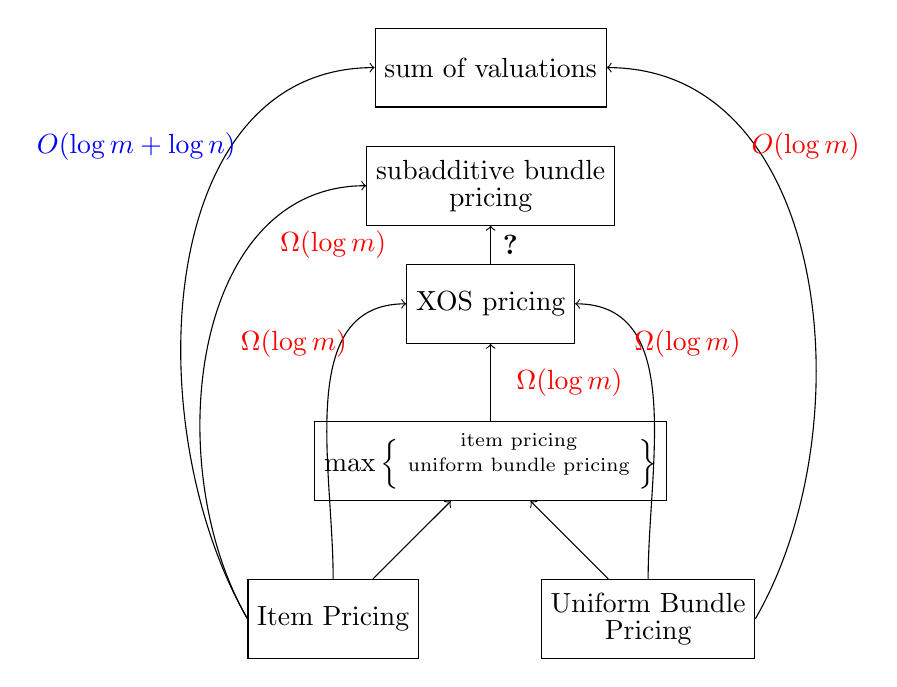
\begin{tikzpicture}
		\node (rectsum) [rectangle, draw, minimum width=7mm, minimum height=10mm] at (0,1.5) {sum of valuations};
		
		\node (rectbundle) [rectangle, draw, minimum width=7mm, minimum height=10mm] at (0,0) {\shortstack{subadditive bundle \\ pricing}};
		
		\node (rectxos) [rectangle, draw, minimum width=7mm, minimum height=10mm] at (0,-1.5) {XOS pricing};
		
		\node (rectmax) [rectangle, draw, minimum width=7mm, minimum height=10mm] at (0,-3.5) {$\max \Big\{$  \shortstack{\scriptsize item pricing \\ \scriptsize uniform bundle pricing} $\Big\}$};
		
		\node (rectitem) [rectangle, draw, minimum width=7mm, minimum height=10mm] at (-2,-5.5) {Item Pricing};
		
		\node (rectubundle) [rectangle, draw, minimum width=7mm, minimum height=10mm] at (2,-5.5) {\shortstack{Uniform Bundle \\ Pricing}};
		
		\draw [->] (rectubundle.east) to [out=60, in = 0] (rectsum);
		\node at (4,0.5) {\textcolor{red}{$O( \log m)$}};
		\draw [->] (rectubundle) to [out=90, in = 0] (rectxos);
		\node at (2.5,-2) {\textcolor{red}{$\Omega( \log m)$}};
		\draw [->] (rectitem.west) to [out=120, in = -180] (rectsum.west);
		\node at (-4.5,0.5) {\textcolor{blue}{$O( \log m + \log n)$}};
		\draw [->] (rectitem) to [out=90, in = -180] (rectxos.west);
		\node at (-2.5,-2) {\textcolor{red}{$\Omega( \log m)$}};
		\draw [->] (rectxos) to  (rectbundle);
		\node at (0.25,-0.75) {\textbf{?}};
		\draw [->] (rectitem.west) [out = 120, in = -180] to  (rectbundle.west);
		\draw [->] (rectmax)  to  (rectxos);
		\draw [->] (rectitem)  to  (rectmax);
		\draw [->] (rectubundle)  to  (rectmax);		
		\node at (-2,-0.75) {\textcolor{red}{$\Omega( \log m)$}};
		\node at (1,-2.5) {\textcolor{red}{$\Omega( \log m)$}};
		
		\end{tikzpicture}
	}
	\caption{Results Summary: Red font show results in this paper; blue font shows existing known results}
	\label{fig:summary}
\end{figure}

\subsection{Uniform Bundle Pricing}

We begin by proving the $O(\log m)$ upper bound with respect to sum of valuations. 

\begin{lemma}
	Consider a hypergraph $\mH = (\mV, \mE)$ with $m$ edges and valuation $v_e$ for each edge $e \in \mE$. Then, there exists a uniform price $p'$ such that $p^{b}_e = p'$ achieves $O(\log m)$-approximation. 
\end{lemma}
\begin{proof}
	Consider the valuations $v_{e_1}, v_{e_2}, \dots, v_{e_m}$ in increasing order. We claim that $ p^{b}_e  = v_{e_{i'}}$ achieves the desired approximation for some edge $e_{i'}$. Assume for the sake of contradiction that this is not the case. Let $\textsf{OPT} = \sum_{e \in \mE} v_e$. Then $m v_{e_1} < \textsf{OPT}/ \log m$ since we can sell each edge if the bundle price is the smallest valuation. Similarly, $(m - i) v_{e_i} < \textsf{OPT}/ \log m$ for each edge. Adding up all inequalities, we get:
	
	\begin{equation}
	\begin{aligned}
	\textsf{OPT} = \sum_{e \in \mE} v_e & < \frac{\textsf{OPT}}{\log m} (\frac{1}{m} + \frac{1}{m-1} + \dots + 1) \\
	& \leq \textsf{OPT}
	\end{aligned}
	\end{equation}
	
	which is a contradiction.
\end{proof}

Next, we show that the $O(\log m)$ upper bound is tight.

\begin{lemma}
	There exists a set of buyers with XOS valuations such that any uniform bundle price produces revenue at most $\textsf{OPT}/ \log m$.
\end{lemma}	
\begin{proof}
	Consider $n=m$ items and $m$ buyers such that buyer $b_i$ wants item $i$ for price $1/i$. It is easy to see that the valuations are XOS and achieves a revenue of $\log m$. Consider any fixed $p^b_e = 1/c$ such that $1 \leq c \leq m$. Then, the seller can sell edges that have valuation at least $1/c$. Observe that the number of such edges is at most $c$. Therefore, the revenue is at most $\sum_{e:v_e \leq 1/c} 1/c = O(1)$.
\end{proof}

\subsection{Item Pricing}

Next, we show the $\Omega(\log m)$ gap between item pricing and XOS pricing.

\begin{lemma}
	There exists a set of buyers with XOS valuations such no item pricing solution can obtain revenue better than $\textsf{OPT}/ \log m$.
\end{lemma}
\begin{proof}
	Let $\mC_i$ denote the class of customers that desire exactly $\vert i \vert$ items. We construct the hypergraph instance as follows: Each class of customers $\mC_i$ has exactly $\lceil n/i \rceil$ and each customer in $\mC_i$ is assigned a partition of $i$ items such that no two customers share any item. Thus, the total number of hyperedges is $m = \sum_{i} \vert \mC_i \vert = \Theta( n \log n)$. Figure shows  an instance for $n=6$. We fix the valuation $v_e = 1$ for all hyperedges. This set of valuations is XOS and the revenue obtained by selling each edge at price $p^{b}_e = 1$ extracts the full revenue of $\Theta(n \log n)$.
	
	Next, we show that no item pricing solution can do better than $O(n)$. We will show this by induction on the customer class $\mC_i$. The base case is revenue obtained by selling edges to customers in $\mC_1$. Since there are at most $n$ edges, the maximum revenue is $O(n)$. Consider the customer class $\mC_k$. Let denote $0 < \alpha \leq 1$ be the fraction of edges sold to customers in $\mC_k$ and let $\mE_k$ denote such edges. Then, the maximum revenue that can be extracted is $\alpha \lceil n/k \rceil$. We distinguish three types of edges: $(i)$ edges that share at least one item with edges in $\mE_k$ $(ii)$ edges that do not share any item with edges in $\mE_k$ $(iii)$ edges that are strictly contained within $\mE_k$. By the induction hypothesis, the maximum revenue that can be extracted from all type $(ii)$ edges is at most $O(n)$. Each edge in $\mE_k$ can overlap with at most $2(k-1)$ edges that have size strictly lesser than $k$. Thus, the revenue extracted from type $(i)$ edges is at most $2(k-1) \alpha \lceil n/k \rceil = O(n)$. Consider an edge $e' \in \mE_k$ and let $w_1, \dots w_k$ be the weights of items in $e'$. Since the seller is able to sell $e'$, we have that $w_1 + \dots w_k \leq 1$. Observe that the maximum revenue of all edges of size strictly lesser than $k$ (say $k'$) using items in $e'$ is also at most $w_1 + \dots w_k \leq 1$ which gives revenue of $O(k)$. 
\end{proof}

\subsection{Lower bound for maximum of item pricing and uniform bundle pricing} \label{sub:sec:maxitembundle}

In this section, we construct an instance where the revenue gap between the optimal subadditive pricing and the optimal revenue obtained from either item pricing or uniform bundle pricing is $\Omega(\log m)$. 

\begin{figure}[t]
	\scalebox{1}{
		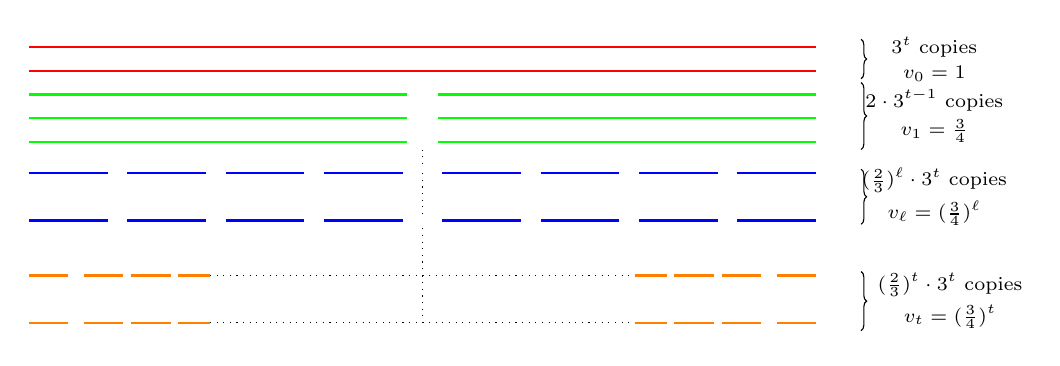
\begin{tikzpicture}
			\draw [red, thick] (-5,5) to (5,5);
			\draw [red, thick] (-5,4.7) to (5,4.7);
			
			\draw [decorate,decoration={brace,amplitude=2pt,raise=2pt},yshift=0pt]
			(5.5,5.1) -- (5.5,4.6) node [black,midway,xshift=1cm] {
				\shortstack{ \scriptsize $3^t$ copies \\ \scriptsize $v_0 = 1$}};
			
			\draw [green, thick] (-5,4.4) to (-0.2,4.4);
			\draw [green, thick] (0.2,4.4) to (5,4.4);
			
			\draw [green, thick] (-5,4.1) to (-0.2,4.1);
			\draw [green, thick] (0.2,4.1) to (5,4.1);			
			
			\draw [green, thick] (-5,3.8) to (-0.2,3.8);
			\draw [green, thick] (0.2,3.8) to (5,3.8);			
			
			\draw [decorate,decoration={brace,amplitude=2pt,raise=2pt},yshift=0pt]
			(5.5,4.55) -- (5.5,3.7) node [black,midway,xshift=1cm] {
			\shortstack{ \scriptsize $2 \cdot 3^{t-1}$ copies \\ \scriptsize $v_1 = \frac{3}{4}$}};			
		
			\draw[dotted]  (0, 3.7) -- (0, 3.45);
			
			\draw [blue, thick] (-5,3.4) to (-4,3.4);
			\draw [blue, thick] (-3.75,3.4) to (-2.75,3.4);			
			\draw [blue, thick] (-2.5,3.4) to (-1.5,3.4);			
			\draw [blue, thick] (-1.25,3.4) to (-0.25,3.4);									
			\draw [blue, thick] (5,3.4) to (4,3.4);
			\draw [blue, thick] (3.75,3.4) to (2.75,3.4);			
			\draw [blue, thick] (2.5,3.4) to (1.5,3.4);			
			\draw [blue, thick] (1.25,3.4) to (0.25,3.4);			
			
			\draw[dotted]  (0, 3.4) -- (0, 2.85);
			
			\draw [blue, thick] (-5,2.8) to (-4,2.8);
			\draw [blue, thick] (-3.75,2.8) to (-2.75,2.8);			
			\draw [blue, thick] (-2.5,2.8) to (-1.5,2.8);			
			\draw [blue, thick] (-1.25,2.8) to (-0.25,2.8);									
			\draw [blue, thick] (5,2.8) to (4,2.8);
			\draw [blue, thick] (3.75,2.8) to (2.75,2.8);			
			\draw [blue, thick] (2.5,2.8) to (1.5,2.8);			
			\draw [blue, thick] (1.25,2.8) to (0.25,2.8);
			
			\draw [decorate,decoration={brace,amplitude=2pt,raise=2pt},yshift=0pt]
			(5.5,3.45) -- (5.5,2.75) node [black,midway,xshift=1cm] {
				\shortstack{ \scriptsize $(\frac{2}{3})^\ell \cdot 3^{t}$ copies \\ \scriptsize $v_\ell = (\frac{3}{4})^{\ell}$}};			
			
			\draw[dotted]  (0, 2.7) -- (0, 2.1);
			
			\draw [orange, thick] (-5,2.1) to (-4.5,2.1);
			\draw [orange, thick] (-4.3,2.1) to (-3.8,2.1);
			\draw [orange, thick] (-3.7,2.1) to (-3.2,2.1);
			\draw [orange, thick] (-3.1,2.1) to (-2.7,2.1);			
			\draw[dotted] (-2.7, 2.1) to (2.7, 2.1)			;
			\draw [orange, thick] (5,2.1) to (4.5,2.1);
			\draw [orange, thick] (4.3,2.1) to (3.8,2.1);
			\draw [orange, thick] (3.7,2.1) to (3.2,2.1);
			\draw [orange, thick] (3.1,2.1) to (2.7,2.1);			
			
			
			\draw[dotted]  (0, 2.1) -- (0, 1.5);
			
			\draw [orange, thick] (-5,1.5) to (-4.5,1.5);
			\draw [orange, thick] (-4.3,1.5) to (-3.8,1.5);
			\draw [orange, thick] (-3.7,1.5) to (-3.2,1.5);
			\draw [orange, thick] (-3.1,1.5) to (-2.7,1.5);			
			\draw[dotted] (-2.7, 1.5) to (2.7, 1.5)			;
			\draw [orange, thick] (5,1.5) to (4.5,1.5);
			\draw [orange, thick] (4.3,1.5) to (3.8,1.5);
			\draw [orange, thick] (3.7,1.5) to (3.2,1.5);
			\draw [orange, thick] (3.1,1.5) to (2.7,1.5);			
			
			\draw [decorate,decoration={brace,amplitude=2pt,raise=2pt},yshift=0pt]
			(5.5,2.15) -- (5.5,1.4) node [black,midway,xshift=1.2cm] {
				\shortstack{ \scriptsize $(\frac{2}{3})^{t} \cdot 3^{t}$ copies \\ \scriptsize $v_{t} = (\frac{3}{4})^{t}$}};			
			
			
		\end{tikzpicture}
	}
	\caption{Laminar family construction for Section~\ref{sub:sec:maxitembundle} lower bound}
	\label{fig:laminar}
\end{figure}


We will construct a laminar family of sets arranged in binary tree fashion as follows: The root node is the set of all $n = 2^{t}$ items. At depth $\ell$, there are $2^\ell$ sets, each of size $\left( \frac{n}{2^{\ell}} \right)$ formed by partitioning each set at depth $\ell-1$ of size $\left( \frac{n}{2^{\ell - 1}} \right)$ into two. Further, each set $S$ at depth $\ell$ has valuation $v(S) = \left( \frac{3}{4} \right)^{\ell}$ and $c_\ell = \left( \frac{2}{3} \right)^{\ell} 3^t$ copies of itself. Figure~\ref{fig:laminar} shows the construction. Let $\mL$ denote the family of laminar sets in the construction and $v(A) = \min_{X \subseteq \mL} \sum_{S \in X} v(S)$ where $X$ is a set cover of $A$ be the pricing function extension. Note that $v(A)$ is monotone and subadditive. 

\begin{lemma}
	Optimal revenue extracted on the instance is $\textsf{OPT} = t \cdot 3^{t}$
\end{lemma}
\begin{proof}
	Consider the revenue extracted by selling sets at any level $\ell$. The are $2^{\ell}$ sets and $(2/3)^{\ell} \cdot 3^{t}$ copies of each set. Thus, the total revenue from all $t$ levels is,
	
	\begin{align*}
	\textsf{OPT} = \sum_{\ell = 0}^{\ell = t} v_\ell c_\ell 2^\ell = \left( \frac{3}{4} \right)^{\ell}  \cdot \left( \frac{4}{3} \right)^{\ell} \cdot  3^{t} = t \cdot 3^{t}
	\end{align*}
\end{proof}

Next, we will show that no uniform bundle pricing or item pricing can extract revenue more than $O(3^{t})$.

\begin{lemma}
	No uniform bundle price can obtain revenue more than $O(3^{t})$
\end{lemma}	
\begin{proof}
	The first observation is that we need to consider only bundle prices of the form $\left( \frac{3}{4} \right)^{k}$. Let the bundle price chosen be $\left( \frac{3}{4} \right)^{k}$. Then, we can sell all edges at depth $\leq k$. This gives us the revenue bound,
	
	\begin{align*}
	\textsf{OPT}_B & = \sum_{i \leq k} \left( \frac{3}{4} \right)^{k} \cdot \left( \frac{2}{3} \right)^{i} \cdot 3^{t} \cdot 2^{i} 
	\displaybreak[0]\\
	& = \left( \frac{3}{4} \right)^{k} \cdot 3^{t} \sum_{i \leq k} \left( \frac{4}{3} \right)^{i} \displaybreak[0]\\
	& \leq \left( \frac{3}{4} \right)^{k} \cdot 3^{t} \cdot \left( \frac{4}{3} \right)^{k} = O(3^{t})
	\end{align*}
	
\end{proof}

\begin{lemma}
	No item pricing can obtain revenue more than $O(3^{t})$
\end{lemma}
\begin{proof}
	Let $k$ be the smallest depth for any set sold by the optimal item pricing solution. The main observation is that the revenue obtained from all sets sold by optimal item pricing is at most the revenue obtained by selling all sets with depth $\geq k$. This is true because we can only overestimate the revenue by considering some sets that are not otherwise part of the item pricing solution. Consider the revenue obtained from all sets at depth $k$. Each set has valuation $\left( \frac{3}{4} \right)^{k}$ and there are $2^{k}$ sets. Observe that the item pricing can hope to extract at most $\left( \frac{3}{4} \right)^{k} \cdot 2^{k}$ revenue from any level $\geq k$.  Thus, the total revenue from all copies of sets with depth $ \geq k$ is,
	
	\begin{align*}
		\textsf{OPT}_{IP} & = \sum_{i \geq k} \left( \frac{3}{4} \right)^{k} \cdot   2^{k}  \cdot  c_i \displaybreak[0]\\
		& = \left( \frac{3}{2} \right)^{k} \cdot   3^{t} \sum_{i \geq k} \left( \frac{2}{3} \right)^{k} \displaybreak[0] \\
		& \leq \left( \frac{3}{2} \right)^{k} \cdot  3^{t+1} \cdot  \left( \frac{2}{3} \right)^{k} \cdot  \left( 1 - \left(\frac{2}{3}\right)^{t - k} \right) \displaybreak[0] \\
		& = O(3^{t})
	\end{align*}
\end{proof}

The last part is to express the revenue gap $\Omega(t)$ in terms of the total number of sets $m$ in the family. Note that $m = \sum_{i = 0}^{i = t} 3^{t} \cdot  2^{k} \cdot  \left( \frac{2}{3} \right)^{k} \leq 3^{t} \cdot  \left( \frac{4}{3} \right)^{t+1} = O(4^{t})$ and thus, the revenue gap is $\Omega(\log m)$. 


\todo{Needs more work}
Next, we will show that the pricing function extension $v(A) = \min_{X \subseteq \mL} \sum_{S \in X} v(S)$ is a submodular function. Before that, we will introduce some more notation. Let $\bA$ denote the minimum weighted set covering of a set $A$, i.e. $\bA = \argmin_{X \subseteq \mL} \sum_{S \in X} v(S)$  where $X$ is a set cover of $A$. We overload the valuation function $v$ to mean $v(\bA) = \sum_{S \in \bA} v(S)$ and define $\bA^{*} = \bigcup_{X \in \bA} X$. For any two sets $A, B \in 2^{[n]}$, it holds that $v(A) + v(B) = v(\bA) + v(\bB)$. Observe that $A \cap B \subseteq \bA^{*} \cap \bB^{*}$ and by monotonicity, we have $v(A \cap B) \leq v(\bA^{*} \cap \bB^{*})$. Similarly, $v(A \cup B) \leq v(\bA^{*} \cup \bB^{*})$. Thus, to show submodularity, it suffices to show that $v(\bA) + v(\bB) \geq v(\bA^{*} \cup \bB^{*}) + v(\bA^{*} \cap \bB^{*})$. We proceed by induction on the height $u$ of the tree and consider sets at height at most $u$ in the minimum covering.


\smallskip
\introparagraph{Base Case} Let $L^{0}_1, \dots, L^{0}_{n} \in \mL$ denote the singleton sets at height $u = 0, \bA_i = \bA \cap L^{0}_i, \bB_i = \bB \cap L^{0}_i$.
\begin{align*}
	v(\bA) + v(\bB) & = v(\bA_1) + \dots + v(\bA_n) +  v(\bB_1) + \dots + v(\bB_n) \displaybreak[0]\\
	& = v(\bA_1) + v(\bB_1) + \dots + v(\bA_n) + v(\bB_n) \displaybreak[0] \\
	& = v(\bA_1 \cap \bB_1) + \dots + v(\bA_n \cap \bB_n) + v(\bA_1 \cup \bB_1) + \dots + v(\bA_n \cup \bB_n) \displaybreak[0]\\
	& = v( (\bA \cap \bB) \cap L^{0}_1) + \dots + v( (\bA \cap \bB) \cap L^{0}_n) +  v( (\bA \cup \bB) \cap L^{0}_1) + \dots + v( (\bA \cup \bB) \cap L^{0}_n) \displaybreak[0]\\
	& \geq v(\bA \cup \bB) + v(\bA \cap \bB) \geq v(\bA^{*} \cup \bB^{*}) + v(\bA^{*} \cap \bB^{*})
\end{align*}

The third equality holds since each $\bA_i$ and $\bB_i$ is either an empty set or singleton, fourth equality holds by definition and last inequality holds by subadditivity.

\smallskip
\introparagraph{Inductive Case} Assume that $v(\bA) + v(\bB) \geq v(\bA^{*} \cup \bB^{*}) + v(\bA^{*} \cap \bB^{*})$ holds for height $u-1$, i.e. when the minimum weighted covering is formed using sets at height at most $u-1$. Consider all laminar sets Let $L^{u}_1, \dots, L^{u}_{n/2^u} \in \mL$ at height $u$  and $\bA_i = \bA \cap L^{u}_i, \bB_i = \bB \cap L^{u}_i$. Using the same argument as in the base case, we have 

\begin{align*}
v(\bA) + v(\bB) & = v(\bA_1) + \dots + v(\bA_{n/2^{u}}) +  v(\bB_1) + \dots + v(\bB_{n/2^{u}}) \displaybreak[0]\\
& = v(\bA_1) + v(\bB_1) + \dots + v(\bA_{n/2^{u}}) + v(\bB_{n/2^{u}}) \displaybreak[0] \\
& \geq v(\bA_1 \cap \bB_1) + \dots + v(\bA_{n/2^{u}} \cap \bB_{n/2^{u}}) + v(\bA_1 \cup \bB_1) + \dots + v(\bA_{n/2^{u}} \cup \bB_{n/2^{u}}) \displaybreak[0]\\
& = v( (\bA \cap \bB) \cap L^{u}_1) + \dots + v( (\bA \cap \bB) \cap L^{u}_{n/2^{u}}) +  v( (\bA \cup \bB) \cap L^{u}_1) + \dots + v( (\bA \cup \bB) \cap L^{u}_{n/2^{u}}) \displaybreak[0]\\
& \geq v(\bA \cup \bB) + v(\bA \cap \bB) \geq v(\bA^{*} \cup \bB^{*}) + v(\bA^{*} \cap \bB^{*})
\end{align*}

However, it remains to be shown that the third inequality is true, i.e. $v(\bA_i) + v(\bB_i) \geq v(\bA_i \cup \bB_i) + v(\bA_i \cap \bB_i)$. If either $\bA_i = L^{u}_i$ or $\bB_i = L^{u}_i$, then the inequality (equality in this case) holds.

Otherwise, if each $\bA_i$ and $\bB_i$ is empty, it means that $\bA_i$ and $\bB_i$ are covered by sets with height $< u$. Define $\bA'_i = \bA_i \cap L^{u-1}_i, \bB'_i = \bB_i \cap L^{u-1}_i$. By the inductive hypothesis, it holds that $v(\bA'_i) + v(\bB'_i) \geq v(\bA'_i \cup \bB'_i) + v(\bA'_i \cap \bB'_i)$ and thus,

\begin{align*}
	v(\bA_i) + v(\bB_i) & = v(\bA'_1) + \dots + v(\bA'_{n/2^{u-1}}) +  v(\bB'_1) + \dots + v(\bB'_{n/2^{u-1}}) \displaybreak[0]\\
	& = v(\bA'_1) + v(\bB'_1) + \dots + v(\bA'_{n/2^{u-1}}) + v(\bB'_{n/2^{u-1}}) \displaybreak[0] \\
	& \geq v(\bA'_1 \cap \bB'_1) + \dots + v(\bA'_{n/2^{u-1}} \cap \bB'_{n/2^{u-1}}) + v(\bA'_1 \cup \bB'_1) + \dots + v(\bA'_{n/2^{u-1}} \cup \bB'_{n/2^{u-1}}) \displaybreak[0]\\
	& = v( (\bA_i \cap \bB_i) \cap L^{u-1}_1) + \dots + v( (\bA_i \cap \bB_i) \cap L^{u-1}_{n/2^{u-1}}) +  v( (\bA_i \cup \bB_i) \cap L^{u-1}_1) + \dots + v( (\bA_i \cup \bB_i) \cap L^{u-1}_{n/2^{u-1}}) \displaybreak[0]\\
	& \geq v(\bA_i \cup \bB_i) + v(\bA_i \cap \bB_i)	
\end{align*}

